\documentclass[runningheads, a4paper]{llncs}

\let\proof\relax
\let\endproof\relax

\usepackage{mathtools,amsmath,amssymb,amsthm,bm,faktor}
\usepackage[linesnumbered, ruled]{algorithm2e}
\usepackage{graphicx}
\usepackage{float}
\usepackage{tikz, pgfplots}
\usepackage{csquotes}
\usepackage{color}
\usepackage{multirow}
\usepackage{booktabs}
\usepackage{enumitem}
\usepackage{csquotes}
\usepackage{cite}
\usepackage{hyperref}
\usepackage{cleveref}
\usepackage{subfiles}
\usepackage{lipsum}
\usepackage{todonotes}
\usepackage{lineno}

\linenumbers

\setlist[enumerate,1]{leftmargin=3em}

% macross
\newcommand{\etal}{\textnormal{et al.}}
\newcommand{\Z}{{\mathbb{Z}}}
\newcommand{\F}{{\mathbb{F}}}
\newcommand{\R}{{\mathbb{R}}}
\newcommand{\pk}{{\mathnormal{pk}}}
\newcommand{\sk}{{\mathnormal{sk}}}

% operators
\DeclareMathOperator{\ord}{ord}
\DeclareMathOperator{\poly}{poly}
\DeclarePairedDelimiter{\floor}{\lfloor}{\rfloor}
\DeclarePairedDelimiter{\abs}{\lvert}{\rvert}
\DeclarePairedDelimiter{\norm}{\lVert}{\rVert}
\DeclarePairedDelimiter{\paren}{(}{)}
\DeclarePairedDelimiter{\bkt}{[}{]}
\DeclarePairedDelimiter{\set}{\{}{\}}
\DeclarePairedDelimiter{\innerprod}{\langle}{\rangle}

% tikz
\usetikzlibrary{shapes.geometric, arrows, chains, fit, tikzmark}
\tikzset{REDBOX/.style = {draw=red, thick, inner ysep=2pt, fit=#1}}

% cref
\creflabelformat{equation}{#2#1#3} % no parenthesis for equation environment

% url
\def\UrlBreaks{\do/\do-}

\begin{document}

	\title{Article Title}
	\titlerunning{Article Title}

	\author{
		Jun Jie Sim \inst{2} \orcidID{0000-0002-3709-6929}
	}
	\index{Sim, Jun Jie}
	\authorrunning{JJ Sim}

	\institute{
		Institute for Infocomm Research, Agency for Science, Technology and Research (A*STAR), Singapore \\
			\email{simjj@i2r.a-star.edu.sg}
		\and
		School of Physical \& Mathematical Sciences, Nanyang Technological University, Singapore \\
			\email{\{junjie005@e.ntu.edu.sg\}}
	}

	\maketitle

	\begin{abstract}

		\keywords{keyword1 \and keyword2}
	\end{abstract}

	\section{Math Environments}

	\begin{definition}
		This is a definition. \label{def1}
		\[ x^n + y^n = z^n \label{eq1} \]
	\end{definition}

	\begin{proposition}
		This is a proposition. \label{prop1}
	\end{proposition}

	\begin{lemma}
		This is a lemma. \label{lemma1}
	\end{lemma}

	\begin{theorem}
		This is a theorem. \label{theorem1}
	\end{theorem}

	\[ 1+1=2 \label{eq3} \]

	\begin{example}
		This is an example. \label{eg1}
	\end{example}

	\begin{table}
		\centering
		\begin{tabular}{lcccc}
			\toprule
			& col $1$ & col $2$ & col $3$ & col  $4$ \\
			\midrule
			row $1$ & $(1,1)$ & $(1,2)$ & $(1,3)$ & $(1,4)$ \\
			row $2$ & $(2,1)$ & $(2,2)$ & $(2,3)$ & $(2,4)$ \\
			row $3$ & $(3,1)$ & $(3,2)$ & $(3,3)$ & $(3,4)$ \\
			\bottomrule
		\end{tabular}
		\caption{This is a table.}
		\label{table1}
	\end{table}

	\begin{table}
		\centering
		\begin{tabular}{cccc}
			& A & B & C \\
			\toprule
			\tikzmarknode{J}I & 1 & 2 & 3 \\
			J & 4 & 5 & 6 \\
			K & 7\tikzmarknode{7} & 8 & 9 \\
			\bottomrule
		\end{tabular}
		\begin{tikzpicture}[overlay,remember picture]
			\node[REDBOX=(J) (7)] {};
		\end{tikzpicture}
		\caption{This is a Tikz Red Box Table}
		\label{tab:redbox}
	\end{table}

	\begin{example}
		\label{eg2}
		This is a second example.
		\[ E=mc^2 \label{eq2} \]
	\end{example}

	\lipsum[3-4]

	\section{Subfiles}
	\subfile{sections/subfile}

	\section{Citations}
	You can cite stuff like \cite{article} and \cite{misc}.
	Combined citations look like this \cite{book,incollection}.

	Use cref for math environments.
	\begin{itemize}
		\item An equation I want to cref \cref{eq1}.
		\item A definition I want to cref \cref{def1}.
		\item A proposition I want to cref \cref{prop1}.
		\item A lemma I want to cref \cref{lemma1}.
		\item A theorem I want to cref \cref{theorem1}.
		\item An algorithm I want to cref \cref{algo1}.
		\item An example I want to cref \cref{eg1}.
		\item A line of code I want to cref \cref{algo1} \cref{line1}.
	\end{itemize}

	Note that autoref does not work properly.
	There is a autoref warning \enquote{No autoref name for \enquote{mycounter}} occurs.
	The recommended fix would be to rename counters.
	See \url{http://tex.stackexchange.com/questions/256672/autoref-does-not-seem-to-be-working-properly} for details.
	However, using cref seems to be simpler.

	% \section{Images}
	% 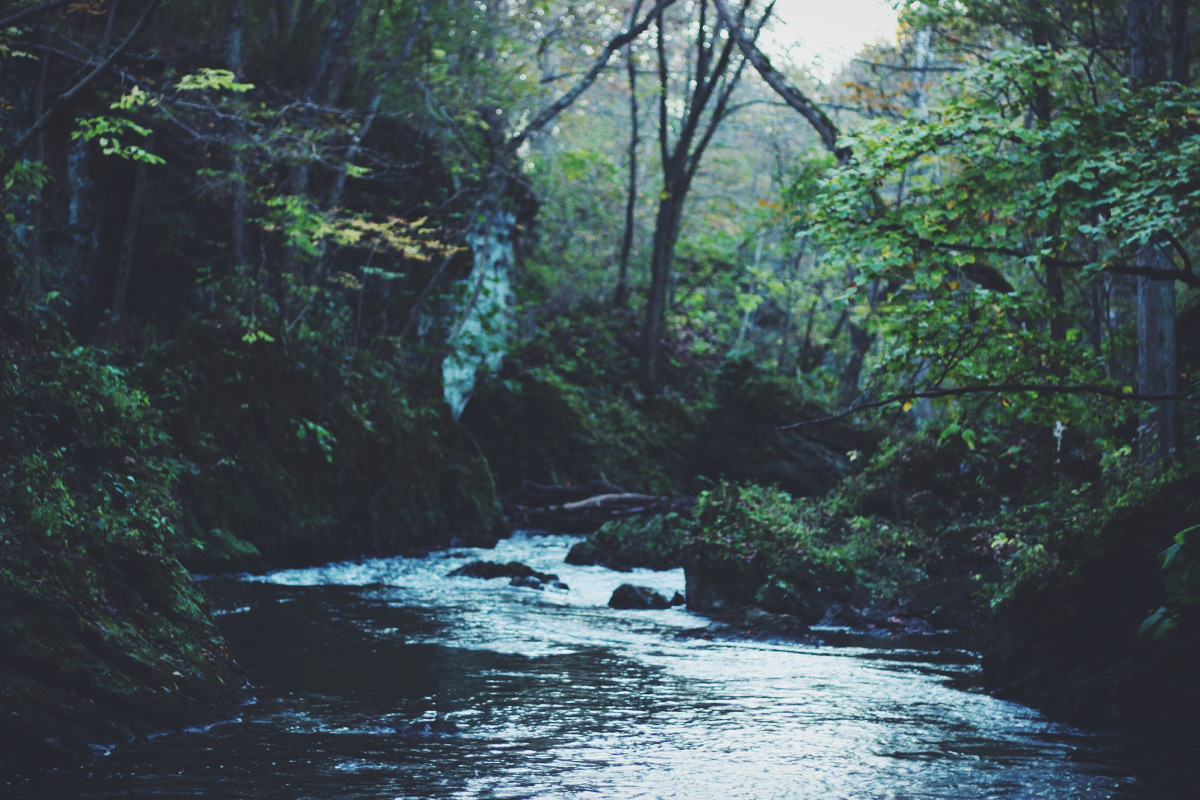
\includegraphics[width=1\textwidth]{stream.jpg}

	% \nocite{*}
	\bibliographystyle{splncs04}
	\bibliography{references}

	% \renewcommand{\appendixname}{Supplementary Material}
	% \appendix
	% \input{z1_results.tex}
	% \input{z2_rmfe_proofs}

\end{document}